\chapter{Estado da arte e viabilidade do proxecto}
\label{chap:arte_viabilidade}

\lettrine{N}{este} segundo capítulo exponse o estado da arte no ámbito das gramolas dixitais. Tamén se fará unha análise da viabilidade do proxecto, deste xeito poderemos determinar se é posible que chegue a finalizarse con éxito.

\section{Estado da arte}
\label{sec:estado_da_arte}
Na actualidade existen diferentes tipos de gramolas, en xeral todas son dixitais e obteñen a información a través de Internet. Hai compañías que ofertan o servizo de obter un aparello físico para dispoñer nun local, e os clientes poidan dun xeito similar a antigamente facer a súa elección musical. Do mesmo xeito existen outras solucións que están baseadas en aplicacións, dunha maneira similar ao noso proxecto, os clientes poden conectarse á estación do lugar onde están e engadir cancións para a súa reprodución. Normalmente estas plataformas contan co seu propio reprodutor de música e o seu propio catálogo, xeralmente bastante extenso pero non tanto coma calquera servizo de música xa que contan coas cancións mais actuais e os clásicos. Non existe un mercado moi amplo aínda que destacan algunhas aplicacións que se están comezando a implantar tanto nos Estados Unidos coma en Europa.\bigskip

Comezando polas gramolas físicas temos a compañía \textbf{TouchTunes}~\cite{touchTunes} que está expandida por Norte América e parte de Europa. Dispoñible en 75.000 bares é a mais coñecida con diferenza, dispón dun gran catálogo de música, sistema de adaptación da música ao local e diferentes ferramentas para o entretemento dos clientes. Oferta de 3 gramolas, dúas de parede, unha que tan só sirve de reprodutor (figura \ref{fig:touchtunes_virtuo}) e outra que contén mais funcionalidades coma o karaoke, unha última adaptable para axeitala o estilo do local coma por exemplo nun barril (figura \ref{fig:touchtunes_fusion}). Todas funcionan con unha gran pantalla táctil para facer a selección, aínda que conta con unha aplicación móbil para este mesmo fin. Utiliza un sistema de créditos que se poden consumir nos diferentes establecementos nos que está implantada a plataforma, polo tanto o seu uso non é gratuíto.

\begin{figure}[hp!]
  \caption{TouchTunes}
  \centering
  \begin{subfigure}[b]{0.3\textwidth}
    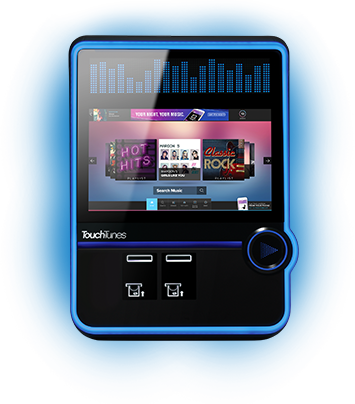
\includegraphics[width=\textwidth]{imaxes/touchtunes_virtuo.png}
    \caption{TouchTunes Virtuo}
	\label{fig:touchtunes_virtuo}
  \end{subfigure}
  \begin{subfigure}[b]{0.3\textwidth}
    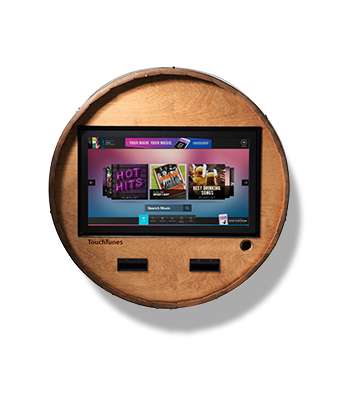
\includegraphics[width=\textwidth]{imaxes/touchtunes_fusion.png}
    \caption{TouchTunes Fusion}
	\label{fig:touchtunes_fusion}
  \end{subfigure}
  \begin{subfigure}[b]{0.2\textwidth}
	  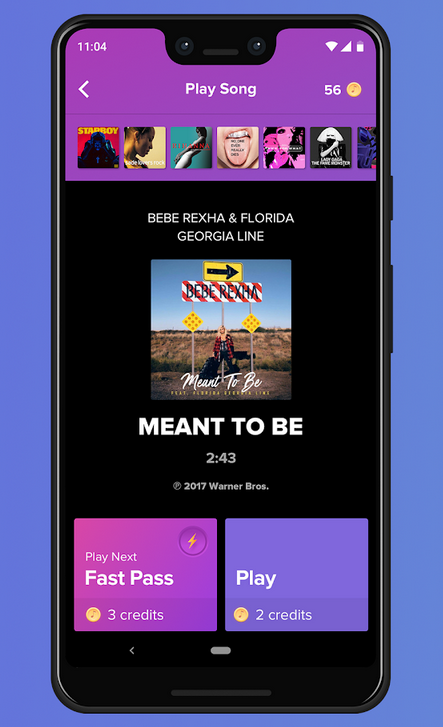
\includegraphics[width=\textwidth]{imaxes/touchtunes_app.png}
	  \caption{Aplicación móbil}
	  \label{fig:touchtunes_app}
  \end{subfigure}
\end{figure}

Como directa competidora de TouchTunes atopamos \textbf{AMI Entertainment}~\cite{amiEntertainment}. Comezou creando pianos nos que introducindo unha moeda podíase elixir algunha das cancións, posteriormente dedicábanse a facer gramolas físicas e nos nosos días seguen coa dixitalización destas. Conta con uns 30.000 aparellos repartidos por todo o mundo. Ao igual que TouchTunes, tamén con 3 tipos de gramolas diferentes, moi similares ás da súa máxima competidora pero inclúen unha de pé (figura \ref{fig:ami_infinity}), similar a unha das gramolas antigas. Tamén conta con aplicación móbil para engadir cancións, e tamén funciona cun sistema de créditos pra facer soar a música que mais che gusta.

\begin{figure}[hp!]
  \caption{Ami Entertainment}
  % \centering
  \begin{subfigure}[c]{0.3\textwidth}
	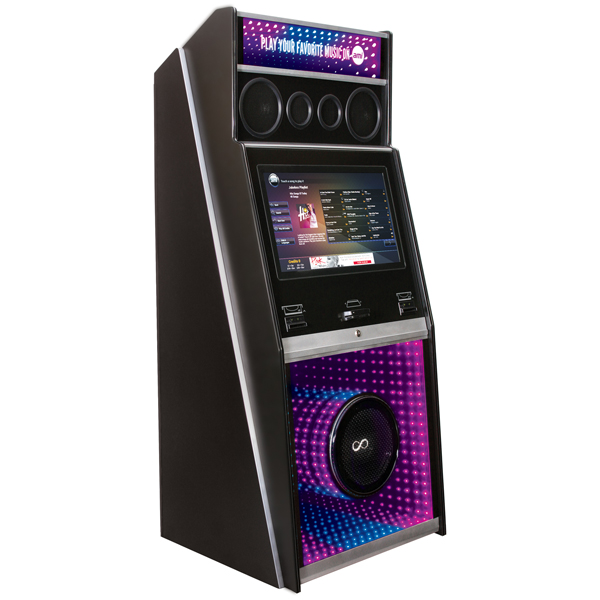
\includegraphics[width=\textwidth]{imaxes/ngx-infinity-ami.jpg}
	\caption{NGX Infinity}
	\label{fig:ami_infinity}
  \end{subfigure}
  \begin{subfigure}[c]{0.5\textwidth}
	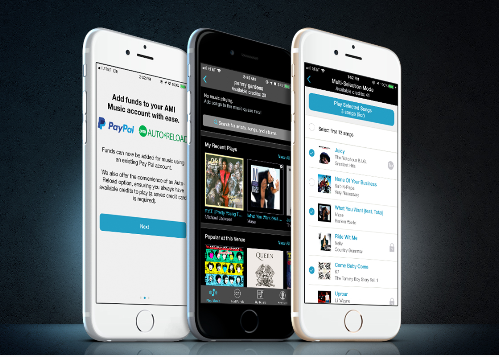
\includegraphics[width=\textwidth]{imaxes/ami_app.png}
	\caption{Aplicación móbil}
	\label{fig:ami_app}
  \end{subfigure}
\end{figure}

No apartado de aplicacións móbil que teñan unha funcionalidade similar a unha gramola atopamos \textbf{Jukestar}~\cite{jukestar}, consiste en dúas aplicacións unha anfitrioa (figura \ref{fig:jukestar_host}) e outra para os invitados (figura \ref{fig:jukestar_jukebox}). O anfitrión ten que conectar a súa conta de Spotify na aplicación e xerar unha festa, despois compartir a sesión de festa cos seus invitados, estes poden incluír cancións ou votar polas da súa preferencia. Estas características funcionan cun sistema de créditos de pago (figura \ref{fig:jukestar_request}). É unha idea similar a da nosa aplicación, xa que utiliza Spotify para a reprodución de música pero necesita un cliente para o anfitrión e outro para os invitados o que complica o seu uso.

\begin{figure}[hp!]
  \caption{Jukestar App}
  \centering
  \begin{subfigure}[c]{0.3\textwidth}
    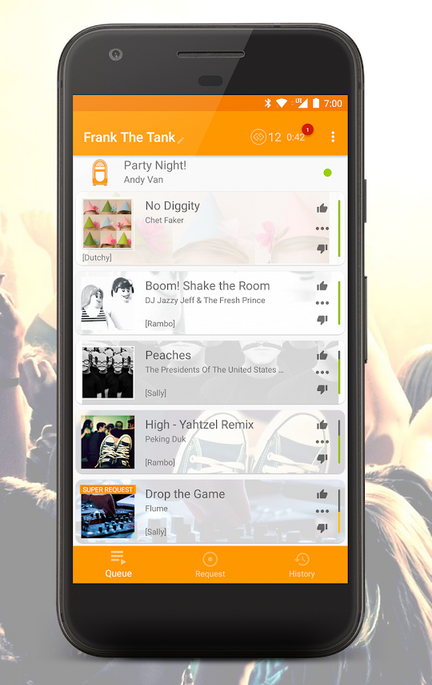
\includegraphics[width=\textwidth]{imaxes/jukestar_jukebox.png}
    \caption{Jukestar gramola}
	\label{fig:jukestar_jukebox}
  \end{subfigure}
  \begin{subfigure}[c]{0.3\textwidth}
    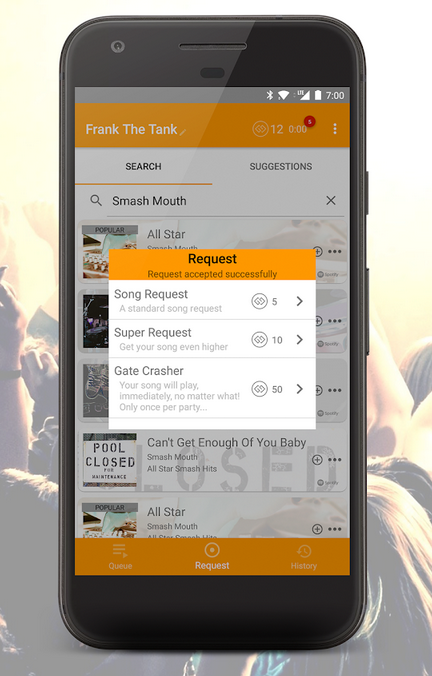
\includegraphics[width=\textwidth]{imaxes/jukestar_request.png}
    \caption{Solicitude de nova canción}
	\label{fig:jukestar_request}
  \end{subfigure}
  \begin{subfigure}[c]{0.3\textwidth}
    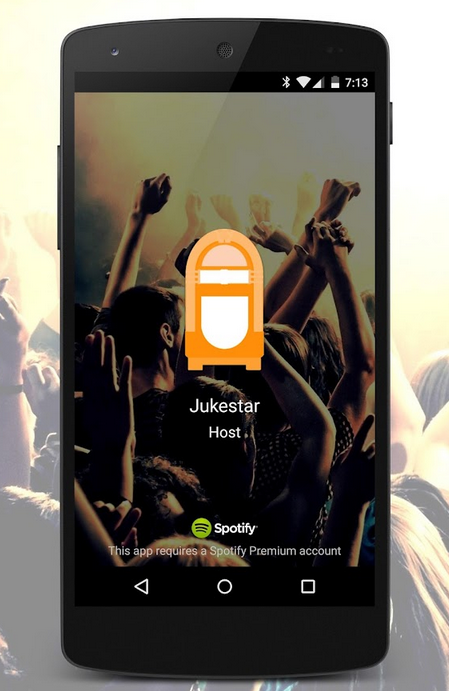
\includegraphics[width=\textwidth]{imaxes/jukestar_host.png}
    \caption{Aplicación anfitrión}
	\label{fig:jukestar_host}
  \end{subfigure}
\end{figure}

Outra aplicación similar é \textbf{Outloud}~\cite{outloud} permite a reprodución de música dende Spotify, SoundCloud e incluso Apple Music para os trebellos compatibles. A idea é similar, créase unha playlist que fai de sesión e os usuarios poden conectarse xa sexa dende un enlace de invitación ou buscando por lugares próximos. Posteriormente poden engadir cancións e votar as que son mais do seu agrado, tamén permite o acceso dende a web sen necesidade de instalar a aplicación. Unha característica que inclúe e non existe noutras aplicacións é a posibilidade de proporcionar información da sesión nunha pantalla central (figura \ref{fig:outloud_screen}), nesta inclúense as seguintes cancións, as cancións acabadas de ser engadidas e incluso quen son os usuarios que reciben mais votos nas súas cancións. Esta aplicación está pensada para usala en calquera lugar: vodas, ximnasios, lugar de traballo, festas particulares, reunións con amigos\dots~ pódese descargar en dispositivos Android ou iOS. Trátase dunha aplicación sinxela ademais de ser gratuíta, o único problema que podemos observar é que a aplicación necesita estar funcionando no dispositivo no que soa a música.

\begin{figure}[hp!]
  \caption{Outloud App}
  \centering
  \begin{subfigure}[c]{0.3\textwidth}
    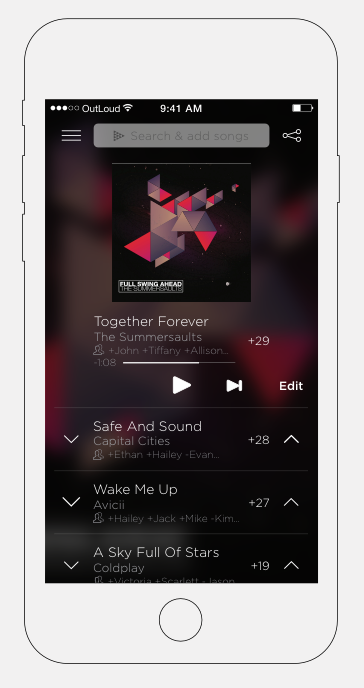
\includegraphics[width=\textwidth]{imaxes/outloud_app.png}
    \caption{Aplicación de Outloud}
	\label{fig:outloud_app}
  \end{subfigure}
  \begin{subfigure}[c]{0.6\textwidth}
    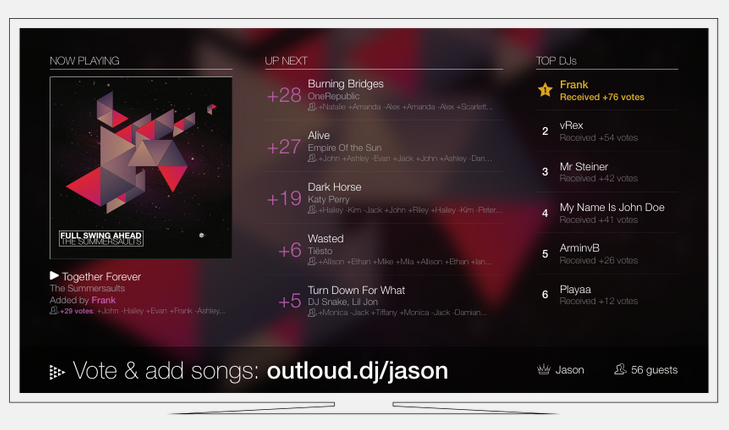
\includegraphics[width=\textwidth]{imaxes/outloud_screen.png}
    \caption{Modo pantalla central}
	\label{fig:outloud_screen}
  \end{subfigure}
\end{figure}

\textbf{Jukebox Today}~\cite{jukeboxToday}, tratase dun servizo web que permite crear sesións e compartilas cos usuarios, non é necesaria unha aplicación como nos servizos anteriores. Permite que a música se reproduza de forma sincronizada en varios dispositivos ou controlar a reprodución dende calquera dos que estea activo, incluso conta con unha sala de conversación para os usuarios. Obtén a música dende YouTube polo tanto o seu catálogo é tan amplo como o da plataforma. Aínda que podería funcionar coma unha gramola non é a súa idea principal, xa que todos os usuarios poden facer modificacións na lista de reprodución ou poñer a pausa, trátase dun servizo gratuíto.

\begin{figure}[hp!]
	\caption{Captura dunha sala en Jukebox Today}
	\centering
	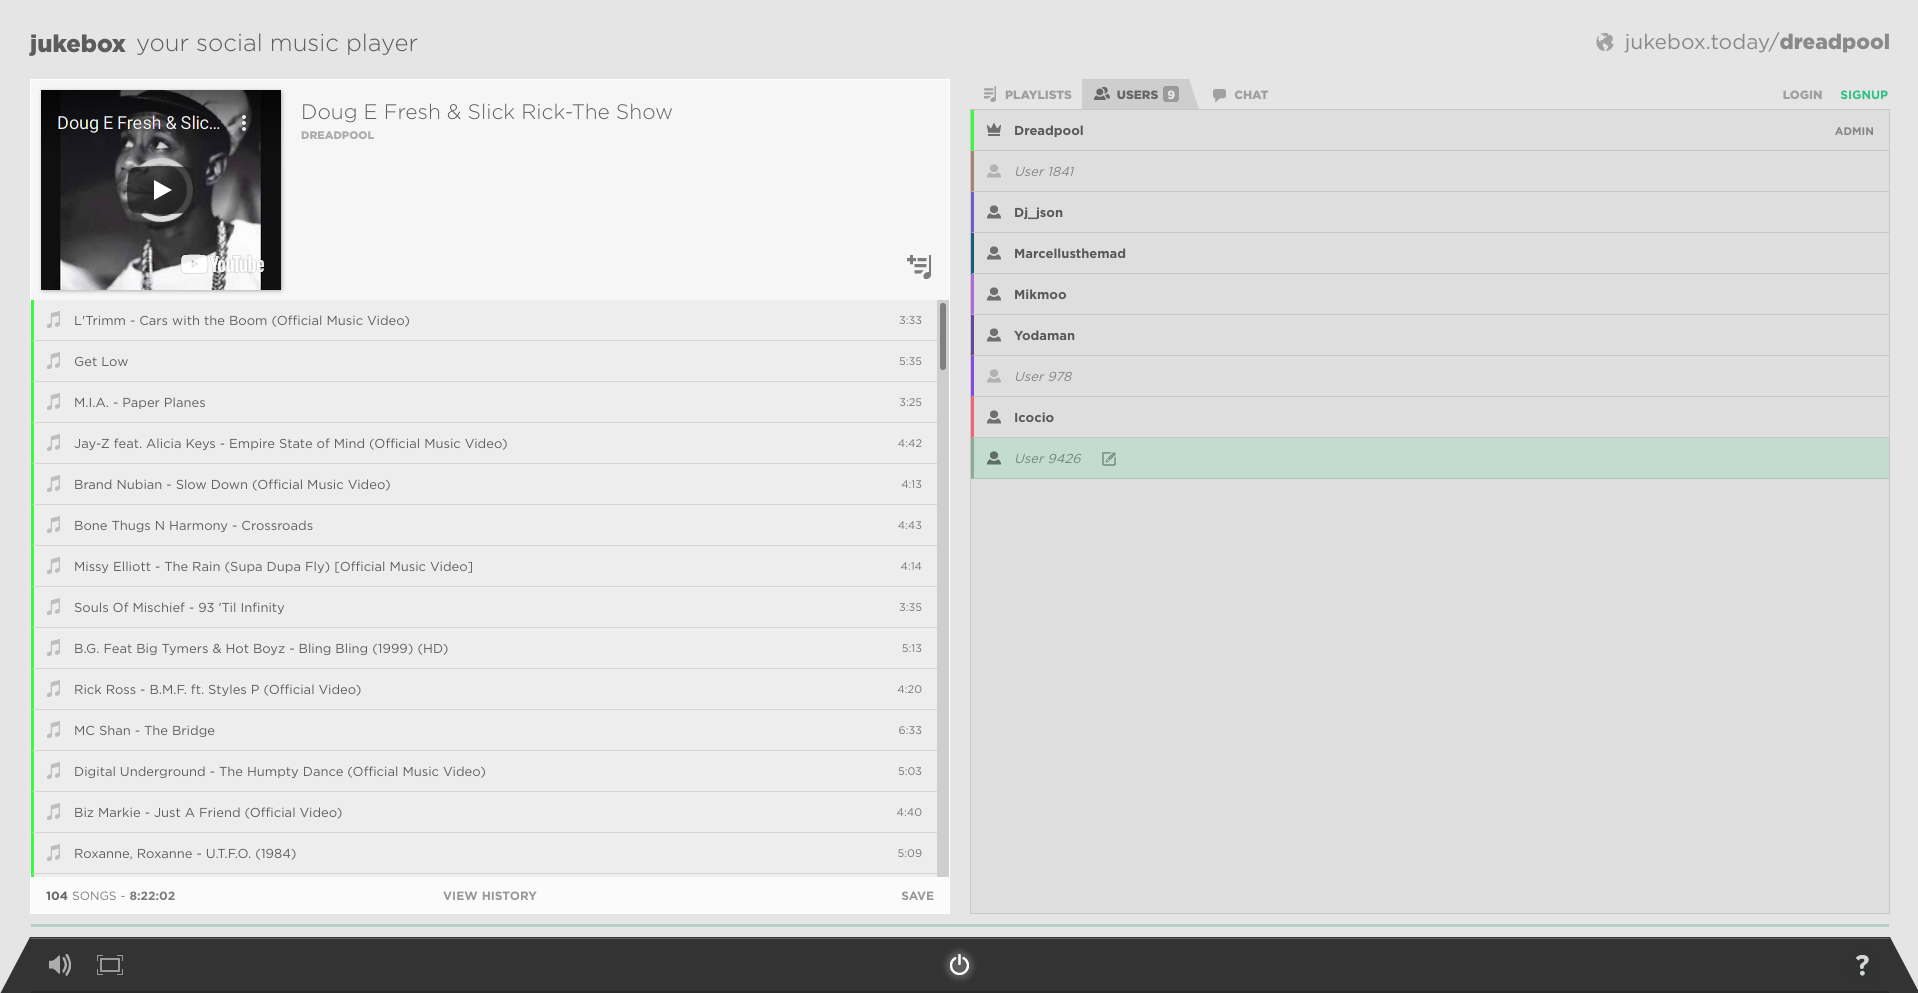
\includegraphics[width=1\textwidth]{imaxes/jukebox_today.png}
	\label{fig:jukebox_today}
\end{figure}

Tamén como servizo web, neste caso de pago atopamos \textbf{BarBox}~\cite{barbox}. Cun prezo de 30 € ao mes para o propietario, pódese dispoñer dun sistema no establecemento onde os clientes tan só necesitan descargar unha aplicación no seu dispositivo e conectarse a rede Wifi. Ademais de contar coas típicas características coma engadir cancións, tamén inclúe un sistema de tokens co que se pode facer que a canción desexada sexa a seguinte en soar. Outra das súas características máis rechamantes é que con tan só estar conectado a rede do local a aplicación solicita as cancións favoritas do usuario.

\begin{figure}[hp!]
  \caption{BarBox App}
  \centering
  \begin{subfigure}[c]{0.3\textwidth}
    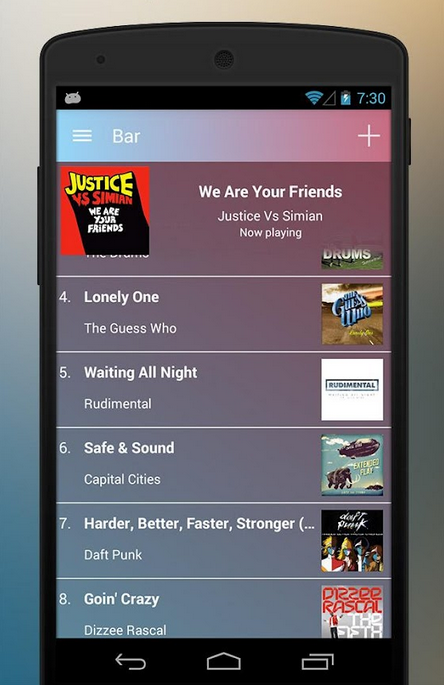
\includegraphics[width=\textwidth]{imaxes/barbox_play.png}
    \caption{BarBox play}
	\label{fig:barbox_play}
  \end{subfigure}
  \begin{subfigure}[c]{0.3\textwidth}
    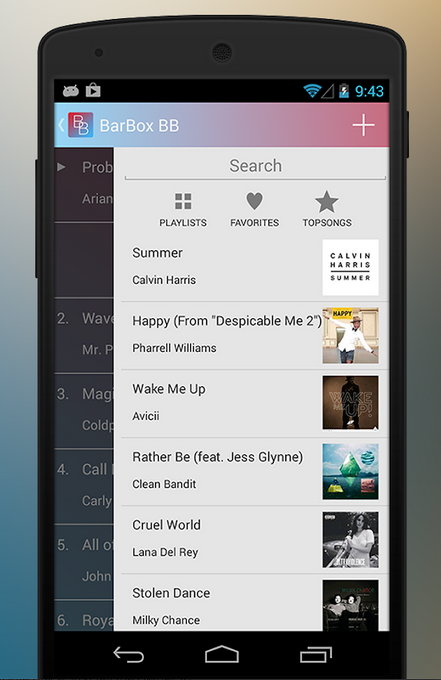
\includegraphics[width=\textwidth]{imaxes/barbox_pick.png}
    \caption{Escoller canción en BarBox}
	\label{fig:barbox_pick}
  \end{subfigure}
\end{figure}

Con funcionamento completamente diferente \textbf{Raveberry}~\cite{raveberry} é un proxecto no que se instala nunha RaspberryPi un servidor musical multiusuario, é dicir, unha gramola. Contén unha interface intuitiva para a solicitude de cancións e cambiar a orde de acordo coa puntuación que os usuarios realizan. Soporta as plataformas de YouTube, Spotify e SoundCloud, incluso permite engadir arquivos locais. Está baseado en Python e contida no repositorio \textit{PyPI} e tamén dispoñible en \textit{Docker} polo tanto é instalable en múltiples dispositivos aínda que é nunha RaspberryPi é onde se poden desfrutar a maioría das súas características que son moitas e moi ben pensadas. Citamos as mais destacadas que converten a Raveberry nun gran proxecto:
\begin{itemize}
	\item \textbf{Streaming remoto:} permite reproducir música sincronizada noutros dispositivos.
	\item \textbf{Bluetooth:} pódese conectar a RaspberryPi a un altofalante Bluetooth que permite evitar os cables.
	\item \textbf{Hotspot:} creación dun punto Wifi no que os usuarios pódense conectar para usar a aplicación ou acceso a Internet.
	\item \textbf{Roles de usuario:} permite engadir permisos a certos usuarios, por exemplo o control da reprodución.
	\item \textbf{Interface gráfica:} o administrador pode elixir a configuración desexada nunha cómoda interface.
	\item \textbf{Shareberry:} é unha aplicación complementaria que permite engadir cancións directamente dende o teléfono móbil.
	\item \textbf{Visualización de pantalla:} usando a aplicación cava, pódense ver as frecuencias de música nunha pantalla conectada \ref{fig:raveberry_visual}.
	\item \textbf{Visualización de son:} pódese engadir dispositivos LED e Raveberry fará que funcionen ao ritmo da música.
\end{itemize}
Para o funcionamento de algunhas destas características é necesaria a inclusión de algún hardware adicional para o que o proxecto xa está preparado. Por exemplo unha antena Wifi para a compartir a conexión, a integración dunha tarxeta de son para a mellora da calidade deste, ou as luces LED que son controladas polos protocolos \textit{i2c} e \textit{spi}. Contén ademais, unha ampla documentación que fai que a súa instalación básica sexa moi sinxela e trátase dun proxecto de código aberto polo tanto gratuíto.

\begin{figure}[hp!]
  \caption{Raveberry Server}
  \centering
  \begin{subfigure}[c]{0.4\textwidth}
    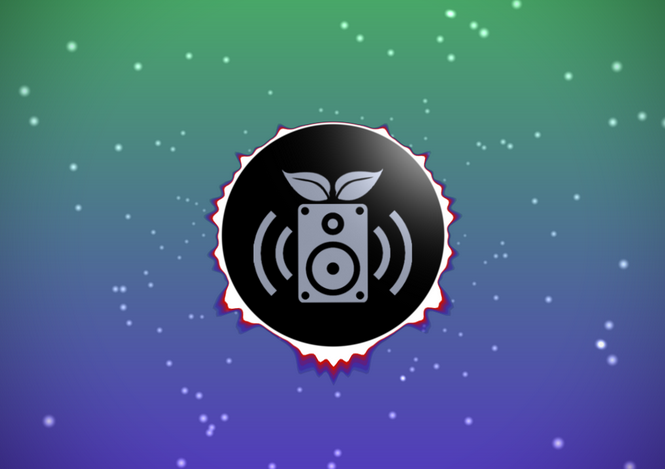
\includegraphics[width=\textwidth]{imaxes/raveberry_logo.png}
    \caption{Visualización de pantalla}
	\label{fig:raveberry_visual}
  \end{subfigure}
  \begin{subfigure}[c]{0.3\textwidth}
    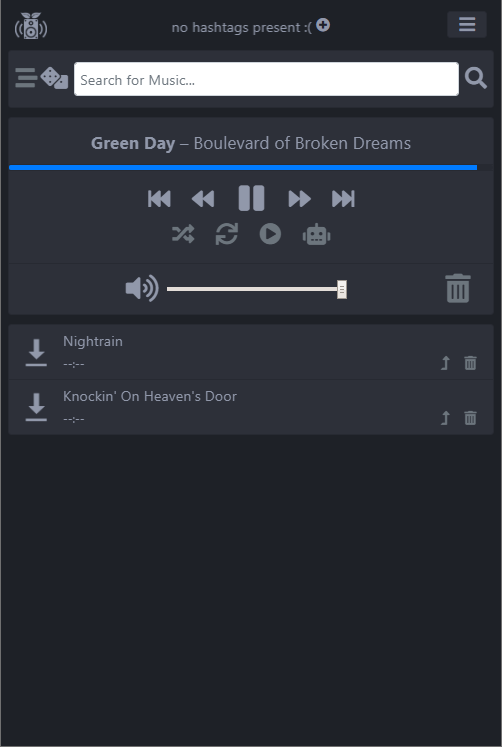
\includegraphics[width=\textwidth]{imaxes/raveberry_interface.png}
    \caption{Interface}
	\label{fig:raveberry_interface}
  \end{subfigure}
\end{figure}

Estes son os proxectos que atopamos cun funcionamento similar ao noso traballo, ningún destes cumpre todos os requisitos aínda que varios aproxímanse a ideas similares. Por exemplo \textit{Outloud} necesita unha aplicación aberta polo tanto no caso de esta estar pechada o servizo deixaría de funcionar, desta forma se dificulta o uso para o administrador. Destes traballos obtivemos ideas que poden ser implementadas no noso proxecto e poden engadir funcionalidades interesantes para o usuario final.

\section{Viabilidade}
Para determinar se o proxecto poderá acadar o seu obxectivo existen varios aspectos a analizar, o conxunto destes é a viabilidade do proxecto. En xeral para os proxectos software as áreas nas que recompilar información para determinar a viabilidade son: técnica, económica, legal e de mercado, deste xeito pódese saber de maneira anticipada cal vai ser o custo aproximado do proxecto, o tempo necesario para rematalo e cal é o impacto no mercado esperado, a continuación descríbense estes diferentes dominios.

\subsection{Viabilidade económica}
Na análise económica téñense en conta tres custos principais, os custos en recursos humanos, en software e en hardware.

Para os \textbf{recursos humanos}, téñense en conta a cantidade de persoas necesarias e o custo por hora de cada unha destas. Neste caso é unha soa persoa a encargada de facer o deseño, implementación e probas. O custo total aproximado é de 460 horas repartidas entre documentación, desenvolvemento, e probas. Na táboa~\ref{tab:custos_humanos} pódese ver en detalle.

Os \textbf{recursos software} teñen en conta os custos do software utilizado para o desenvolvemento do proxecto. Neste proxecto utilízase software libre e gratuíto na maior medida posible, partindo do sistema operativo ata os frameworks e librarías, pasando polas ferramentas de desenvolvemento coma o editor de texto ou o navegador coma veremos mais adiante (sección \ref{sec:ferramentas_desenvolvemento}). Todo isto fai que os custos software neste proxecto sexan nulos, a excepción da necesidade de unha subscrición ao servizo \textit{premium} de Spotify. Na táboa~\ref{tab:spotify_plans} podemos observar os diferentes prezos do servizo, neste caso o plan elixido é o mensual polo tanto o custo ascende a 9,99 € mensuais e aproximadamente de 50 € durante a realización do proxecto.

\begin{table}[tbp]
	\caption{Custos dos plans de Spotify}
	\label{tab:spotify_plans}
	\centering
	\begin{tabular}{|c|c|c|c|c|}
		\hline
		{\textbf{Nome}}             & Individual & Duo    & Familiar & Estudantes \\ \hline
		{\textbf{Número de contas}} & 1          & 2      & 6        & 1          \\ \hline
		{\textbf{Prezo mensual}}    & 9,99 €     & 12,99 €& 15,99 €  & 4,99 €      \\ \hline
		{\textbf{Prezo por conta}}  & 9,99 €     & 6,50 € & 2,67 €   & 4,99 €      \\ \hline
	\end{tabular}
\end{table}

En canto aos \textbf{recursos hardware}, non foi necesario adquirir ningún tipo de equipo, xa que para o desenvolvemento o único necesario é un ordenador con conexión a Internet. Sopesouse a idea de necesitar un servidor na nube para despregar a aplicación o completo, pero debido ao pequeno tamaño da aplicación poderíase recorrer a un servizo gratuíto se fose necesario.

Polo tanto dedúcese que respecto a viabilidade económica este proxecto é completamente factible xa que os custos vense moi reducidos incluso os necesarios son asumibles xa que o servizo \textit{premium} de Spotify é algo que ten mais utilidades que o desenvolvemento.

\subsection{Viabilidade técnica}
A viabilidade técnica é a referente a o funcionamento do sistema, condiciona se as características tecnolóxicas permiten que o proxecto acade un fin exitoso. Neste caso o software escollido para o desenvolvemento aínda que sendo relativamente novo é altamente coñecido e empregado na creación de proxectos similares. Ademais disponse de moita documentación e moi completa, incluso titoriais específicos, o que facilita a realización do proxecto, polo tanto non presenta unha dificultade técnica alta. Respecto ao uso de Spotify como plataforma de reprodución observase que a API é bastante completa, pero non contén peticións para manexar as cancións da cola de reprodución, polo que incrementará a dificultade. Xuntando estes motivos, afírmase que o proxecto é viable tecnicamente.

\subsection{Viabilidade legal}
A nivel legal habería que ter en conta os lugares onde se reproduza a música, isto non é posible controlalo xa que é o usuario final o responsable, polo que non se ten en conta. Si que é importante prestar atención aos termos e condicións de uso da plataforma da que se recolectan as cancións, neste caso especifícase que Spotify é para uso persoal e non comercial polo que quedaría excluído o uso coma gramola nun bar. Considerando que é o usuario final o que decide onde vai utilizar a plataforma, non se considera que exista un problema legal de uso nin que a aplicación incumpra os termos e condicións de uso de Spotify.

\subsection{Viabilidade do mercado}
No apartado do estado da arte \ref{sec:estado_da_arte} observouse que existen diferentes compañías que comercializan gramolas virtuais físicas para establecementos onde se pode engadir música directamente dende un aparello. Estas compañías atópanse algo implantadas en Norte América e comezan a popularizarse en Europa. En canto a software libre, non existen opcións comerciais que cumpran este fin dun xeito similar, e o que existe é tedioso de instalar e máis complexo para o administrador. Tan só hai algúns proxectos ou aplicacións móbiles que de forma xeral crean unha gramola virtual de maneira local para que os usuarios poidan engadir cancións. Incluso Spotify ten unha función de crear unha sesión para compartir con catro usuarios mais, pero que non é tan doado de utilizar en espazos mais grandes, xa que está plantexada para utilizar en pequenas reunións ou lugares con poucos usuarios. Non se atopou ningún proxecto que permita crear unha gramola virtual sen manter outra aplicación funcionando que ademais sexa distribuído de forma gratuíta. Por estes motivos pódese afirmar que este proxecto ten cabida no mercado, entón pode ser consideralo coma viable.\bigbreak

Poñendo en conxunto as distintas análises de viabilidade pódese resumir que o proxecto ten cabida no mercado, é viable economicamente e tecnicamente. Polo tanto dedúcese que o proxecto é viable e é posible que teña éxito no mercado.
